\label{s9} 

%\ssn{Learning Outcomes}
%After studying this week you will be able to:
%\begin{itemize}
%\item calculate probabilities and marginal densities from joint densities;  
%\item use joint densities to solve some problems involving more than one random variable. 
%\end{itemize}
%\end{n}

\subsection{Joint densities}



\ssn{Motivating problems}
\begin{itemize}
\item How can we work with several random variables at once? 
\item A unit length, thin rod breaks in two places, each break independently uniformly distributed on $(0,1)$.  What is the probability that the breaks are more than distance $0.5$ apart? 
\item I choose five numbers in $[0,1]$ uniformly randomly. What is the expected position of the second smallest number? 
\end{itemize}
\end{n}



\ssn{Magic coins}
\begin{table}[h] 
\centering  \[  \arraycolsep=6pt\def\arraystretch{2.0} 
\begin{array}{|c|cc|}
 \hline 
   & X=H & X=T \\ 
  \hline
Y=H &  \frac4{12} & 
      \frac1{12}    \\
Y=T &  \frac2{12} & \frac5{12}  \\
\hline
\end{array} \quad 
\begin{array}{|c|cc|}
 \hline 
   & \PP(X=H)=\frac12 & \PP(X=T)=\frac12 \\
  \hline
\PP(Y=H)=\frac5{12} &  \frac4{12} & 
      \frac1{12}    \\ 
\PP(Y=T)=\frac7{12} &  \frac2{12} & \frac5{12}  \\
\hline
\end{array}
\] 
\caption{Pair of magic coins. (The numbers mean that e.g.\ the probability of both being T is $5/12$.) On the left the probability of all the outcomes is given. In the version on the right the ``marginal probabilities'' for $X$ and $Y$ have been added. \label{mc1}}
\end{table}

My two magic coins $X$ and $Y$ come down with probabilities as in the left-hand side of Table~\ref{mc1}; the four probabilities add up to $1$, as they should.   From that data, we can compute the probabilities that each of the coins separately comes down H or T by adding up each row and column; that information has been added to the table on the right.   But $\PP( \text{$X=H$ and $Y=H$}) \not= \PP(X=H)\, \PP(Y=H)$: the first coin and the second are not independent. 
\end{n}

\ssn{The discrete case}  \label{jdisc} 
Consider two discrete random variables $X,Y$ which for simplicity we assume take values in the non-negative integers $0,1,2,\dots$.   (Each may take infinitely many values (e.g.\ geometric or Poisson) or just a finite number of them (e.g.\ binomial).) 

\tcb 
The \emph{joint probability mass function} of $X,Y$ is 
 \[
      p_{X,Y}(x,y) = \PP(\text{$X=x$ and $Y=y$}). 
 \]
 \etcb 
 
 \noindent
To be valid, we need only to know that 
  \[
    0 \leq p_{X,Y}(x,y) \leq 1 \;\text{ for all $x,y$ } \quad \text{ and } \quad \sum_x \sum_y p_{X,Y}(x,y) = 1. 
   \] 
 
\tcb 
The \emph{marginal mass functions} of $X,Y$ are defined by 
 \[
     p_X(x) = \sum_y p_{X,Y}(x,y)  \quad \text{ and } \quad  p_Y(y) = \sum_x p_{X,Y}(x,y). 
 \]
 \etcb 
 
 \noindent
 They tell us the distribution of each variable, ignoring the other one. 
Clearly, one can extend the definitions to three or more random variables. 
\end{n}

\sse{} 
Prove that the joint mass function $p_{X,Y}$ satisfying the two conditions in \S\ref{jdisc} implies that the marginal distributions satisfy the conditions to be probability mass functions.  
\end{e}

\ssn{The continuous case}
For one continuous random variable $X$ we have a density function $f_X(x)$. It is such that in the limit as  $\Delta x \map 0$ we have 
 \[
    \PP( x \leq X \leq x + \Delta x ) = f_X(x) \Delta x. 
 \]

Two continuous random variables $X,Y$ can be thought of as defining a random point $(X,Y)$ in the plane. A continuous random variable is described by a probability density function $f_{X,Y}$ taking non-negative values so that in the limit as $\Delta x \map 0$ and $\Delta y \map 0$ we have 
 \[
    \PP( \text{$x \leq X \leq x + \Delta x$ and 
    $y \leq Y \leq y + \Delta y$}) = f_X(x,y) \Delta x \Delta y. 
 \]

With our usual convention that the density function is taken to be zero outside of the region where $(X,Y)$ takes values, we require that 
 \[
      \int \int_{\mathbb R^2} f_{X,Y}(x,y) \, \dd x \dd y = 1
 \]
One case is where $f_{X,Y}(x,y) = k$ for all points in some region $D$ in the plane and zero outside. 
This corresponds to choosing a point $(X,Y)$ uniformly randomly in the region $D$.  The constant in that case is $k= 1/\mathop{Area}(D)$ and the probability that $(X,Y)$ lies in a particular (sensibly-shaped) region  $A \subseteq D$ is 

\tcb
 \[
  \PP( (X,Y) \in A) = \frac{\mathop{Area}(A)}{\mathop{Area}(D)}.
  \]
\etcb 
\end{n}

\ssn{Example} 
Let $D$ be the disc of radius $R>0$ centred at the origin and suppose $(X,Y)$ is uniformly distributed in $D$.  Then the probability that $(X,Y)$ lies in the region of the disc given by $x>0$ is $1/2$ and the probability that it lies in the disc of radius $R/2$ centred at the origin is 
 \[
       \frac{\pi (R/2)^2}{\pi R^2} = \frac14. 
  \]
\end{n}

\sse 
A standard dartboard has a scoring area which is a disc of radius 170mm. Between radii of 99 and 107 mm there is an annulus where darts score ``treble''.  One twentieth of that region is the sought-after ``treble 20''.  (Google for a picture of a dartboard -- you are looking for the small red area about 100mm above the centre.)   If darts land uniformly distributed on the scoring area, what is the probability of a ``treble 20''? 
(Ans: 0.0028)
\end{e}

\sss
 The annulus between radii of 99 and 107 has area $\pi(107^2 - 99^2)$ sq mm.  Take one twentieth of that and divide through by the area of the whole board ($\pi 170^2$). 
\end{s}

\sse{} 
In the magic coins example, show that $\PP(X=H \st Y=H) = 4/5$ and compute some other conditional probabilities. 
\end{e}

 \sss 
 Substitute in to $\PP( X=H \text{ and } Y=H) = \PP(Y=H) \PP(X=H \st Y=H)$. 
 \end{s} 



\ssn{The beta distribution} 
We turn now to a related problem which introduces the important beta distribution.  This is not core for us (and so identifying occasions for its use, etc, will not be examined), it provides a good example and is worth being aware of. 
\end{n}

\ssn{Mathematical background}   \label{intfact}
Let $a,b$ be non-negative integers.  Then 
 \[
   I_{a,b} \stackrel{\text{def}}{=}  
   \int_0^1 x^{a-1} (1-x)^{b-1} \dd x = \frac{(a-1)! (b-1)!}{(a+b-1)!} = \frac{\Gamma(a) \Gamma(b)}{\Gamma(a+b)}. 
 \]
To establish this, first check with a trivial integration that $I_{a,1}= 1/a$. Then integrate by parts (differentiating the ``$x^{a-1}$'' term) to establish that 
 \[
     I_{a-1,b} = \frac{b-1}{a-1} I_{a,b-1}.
 \]
With this, we can compute $I_{a,2}$ for all $a$ and so on. 
Thus the two facts 
 \[
      I_{a,1}= \frac1a , \quad I_{a-1,b} = \frac{b-1}{a-1} I_{a,b-1}
 \]
determine $I_{a,b}$ for all positive integer values of $a,b$.  It is easy to check that 
 \[
    B(a,b) =  \frac{\Gamma(a) \Gamma(b)}{\Gamma(a+b)}    
 \]
satisfies the same properties and so is the same function.  (The function $B(a,b)$ is often called the ``beta function''.) 
\end{n}




\ssn{The Beta distribution}
Given that fact, we can define a family of random variables on $[0,1]$. We say that $X$ has a \emph{Beta distribution with parameters $\alpha, \beta \in \mathbb N$} if it has pdf
\[
    f_X(x) =   \frac{\Gamma(\alpha+\beta)}{\Gamma(\alpha) \Gamma(\beta)}  x^{\alpha-1}  (1-x)^{\beta -1}, \qquad x \in [0,1]. 
\]
We will concentrate on the case where $\alpha,\beta$ are positive integers but more generally, everything we have said is true if they are arbitrary positive real numbers. 
\end{n}

\ssn{A problem}
We will now consider the following problem. Consider $n$ points independently uniformly distributed on $[0,1]$. What can I say about where the $k$-th largest point is? 
\end{n}

\ssn{The case $n=2$} 
The first non-trivial instance of the problem is to ask for the distribution of 
 \[
  M_1  = \min(X_1,X_2), \quad M_2 = \max(X_1,X_2)
  \]
 where $X_1, X_2$ are independently uniformly distributed on $[0,1]$. 
 
 Let $\Delta x, \, \Delta y$ be small and consider the probability that $(M_1,M_2)$ lies in the small rectangle where $x \leq M_1 \leq x + \Delta x$ and $y \leq M_2 \leq y+\Delta y$.  We have  
  \[
    \PP(  \text{$x \leq M_1 \leq $ and $y \leq M_2 \leq y+\Delta y$}  ) = f_{M_1,M_2}(x,y) \Delta x \, \Delta y
\]
where $f_{M_1,M_2}(x,y)$ is the joint distribution function. 

We know that $M_1 \leq M_2$ always and so $f_{M_1,M_2}(x,y)=0$ if $x > y$.   If $x \leq y$ however there are two ways that we can have $M_1=x$ and $M_2=y$: either $X_1=x$ and $X_2=y$ or $X_1=y$ and $X_2=x$.  So we have
 \begin{multline*} 
 \PP( (M_1,M_2) \in [x, x+\Delta x] \times [ y,y+\Delta y] )\\  = \PP( (X_1,X_2) \in [x, x+\Delta x] \times [ y,y+\Delta y] ) + \PP( (X_1,X_2) \in [y, y+\Delta y] \times [ x,x+\Delta x] ). 
 \end{multline*} 
 Switching to density functions, still maintaining $x\leq y$ we have 
  \[
     f_{M_1,M_2} (x,y) \Delta x \Delta y 
      =  f_{X_1,X_2} (x,y) \Delta x \Delta y  +
       f_{X_1,X_2} (y,x) \Delta x \Delta y 
  \] 
 and so finally
  \[
     f_{M_1,M_2} (x,y) = \begin{cases}  
            2 &   \text{if $x \leq y$ and $0 \leq x,y \leq 1$}\\
            0 & \text{otherwise}
      \end{cases} 
  \]
Thus $(M_1, M_2)$ is uniformly distributed over the triangle $T$ with vertices $(0,0)$, $(0,1)$ and $(1,1)$ in the $(x,y)$ plane. 

We can also compute the marginal density $f_1(x)$ for the position of $M_1$.  The cumulative distribution $F_1(x)$ is
 \[
  F_1(x) =   \PP( \min(X_1,X_2) \leq x) = 
     \PP( \text{ $X_1=x$ or $X_2=x$}) = 1 - (1-x)^2
 \]
as one can see by drawing a picture. So 
 \[
     f_1(x) = F_1'(x) = 2(1-x). 
 \]
\end{n}

\sse{} 
Compute the density $f_2(x)$ for the position of $M_2$.  Find also $\EE(M_1)$ and $\EE(M_2)$.  (Solution: $f_2(x) = 2x$, $\EE(M_1) = 1/3$, $\EE(M_2) = 2/3$.) 
\end{e} 



\ssn{The general problem}
Let us now solve the problem of the probable location of the k-th smallest point of $n$ points $X_1, \dots , X_n$ independently, uniformly distributed on $[0,1]$.  Let $f_{k,n}(x)$ be the pdf of its location and let $M_k$ be the position of the $k$-th smallest particle  We know that to first order in $\Delta x$ we have 
 \[
   f_{k,n}( x) \Delta x = \PP( x \leq M_k \leq x + \Delta x).
 \]
We now calculate the probability on the right, neglecting and terms involving $(\Delta x)^2$ or higher powers. We do this in two stages.
 \begin{itemize}
     \item There needs to be a point in the interval $[x,x+\Delta x]$. Each point is in the interval with probability $\Delta x$ and there are $n$ points. Thus the probability of this is $n \Delta x$.    (Note: corrections involving two or more points in this interval would involve higher powers of $\Delta x$ and so are discounted.) 
     \item There need to be $k-1$ of the other $n-1$ points lying in the interval $[0,x]$.  This is a binomial distribution problem and the required probability is 
      \[
           \binom{n-1}{k-1} x^{k-1} (1-x)^{n-k}. 
      \]
      This is going to be multiplied by $n \Delta x$ and so any terms here involving $\Delta x$ can be neglected.  (For instance, the uncertainty as to whether one of the $n-k$ particles might actually lie in $[x, x+ \Delta x]$ can be neglected. 
 \end{itemize}
 
Combining these and cancelling $\Delta x$ we arrive at 
\[
    f_{k,n}(x) = \frac{n!}{(k-1)! (n-k)!} x^{k-1} (1-x)^{n-k}
 \]
which we recognise as a Beta distribution with parameters $\alpha=k$ and $\beta = n-k+1$. 
\end{n}

\begin{figure}[h] 
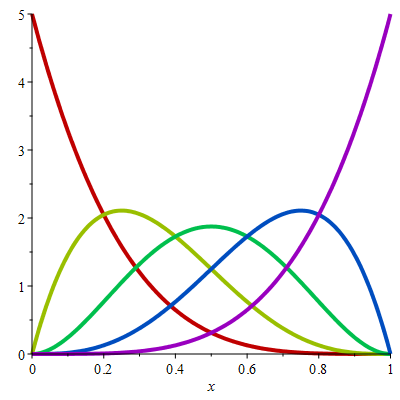
\includegraphics[width=0.45\textwidth]{images/beta5.png}\quad 
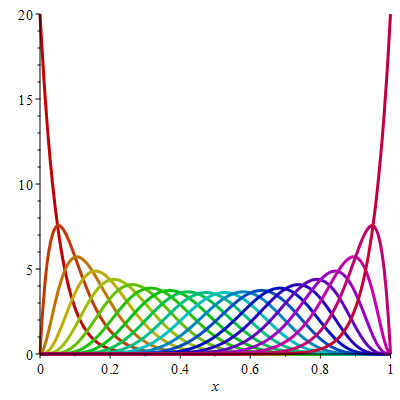
\includegraphics[width=0.45\textwidth]{images/beta20.png}
\caption{Pdf of position of $k$-th smallest of 5 (left) and 20 (right) independent, uniformly distributed numbers in $[0,1]$.  \label{kptpic}}
\end{figure}



\subsection{Exercises} 

\sse 
I toss a fair coin four times. Let $H$ be the number of heads I roll and let $C$ be the number of times (out of the three possible ones) that two consecutive coins tosses give the same result. 

Work out the $5 \times 3$ table of the joint probability mass function. From that compute the marginal distribution of $C$ and check that the marginal distribution of $H$ is binomial as you would expect.   Compute the expected value of $C$.  How could you compute the expected value of $C$ from the initial problem in your head? 
\end{e}

\sse
A unit length, thin rod breaks in two places, each break independently uniformly distributed on $[0,1]$. Let $a$ be a small number. Show that the probability that one of the three pieces into which the rod breaks has length less than $a$ is approximately $6a$ as $a \map 0$. 
\end{e}

\sss 
The relevant regions of the unit square are the four strips of width $a$ along each edge and a strip of width $\sqrt{a}$ around the $X_1 = X_2$ diagonal.  Ignoring overlaps (as $a \map 0$) they have a total area of $6 a$ 
\end{s}

\sse 
Compute the expected position of the $k$-th largest of $n$ independent, uniformly distributed numbers in $[0,1]$.  
\end{e}

\sss 
From the notes the pdf for the $k$th smallest of $n$ is 
\[
    f_{k,n}(x) = \frac{n!}{(k-1)! (n-k)!} x^{k-1} (1-x)^{n-k}. 
 \]
So its expected value is obtained by multiplying by $x$ and integrating: 
 \[
   \EE(X_{k,n}) = \int_0^1  \frac{n!}{(k-1)! (n-k)!} x^{k} (1-x)^{n-k}
   =  \frac{n!}{(k-1)! (n-k)!} \int_0^1   x^{k} (1-x)^{n-k}.
  \]
Using \S\ref{intfact} we evaluate the integral to be 
 \[
 \frac{n!}{(k-1)! (n-k)!} \, \frac{k! (n-k)!}{(n+1)!} = \frac{k}{n+1}.
 \]
\end{s}

\ssp 
Looking at the graphs in Figure~\ref{kptpic}, explain the following features, using mainly words rather than formulas. 
\begin{itemize}
\item Each picture is symmetric about the midpoint of the interval.
\item In the left-hand picture, the central blue-green graph is itself symmetric about the mid-point.
\item In both pictures, two of the graphs have non-zero values at one of the endpoints, but all the rest are zero at both end-points. 
\end{itemize}
\end{e}

\sss
\begin{itemize}
\item This is because the $k$-th smallest particle becomes the $k$-th largest particle if you reflect the interval in the mid-point. 
\item if there are an odd number $2k+1$ of particles, then the $k+1$-th particle reflects to itself under the symmetry just mentioned. 
\item The probability of having one particle in the interval $[0,\Delta t]$ is $n \Delta t$ as $\Delta t \map 0$.  So the corresponding distribution function approaches $n$ at the endpoints. But the probability of two points in such an interval is proportional to $(\Delta t)^2$ and so the distribution function must be zero at the end points. 
\end{itemize}
\end{s}



\subsection{Minimum and Maximum of Random Variables}

\ssn{Motivation}
In a large room are $n$ light bulbs. The owner is a little miserly and only changes them when all have burned out. How long is it till this has happened?
\end{n}

\ssn{Maximum of Random Variables}
Let $X_i$, $i \in \{1,2,\ldots, n \}$ be i.i.d. random variables with cdf $F_X$. 
Then
\begin{align*}
    F_{\max_i X_i} (x)
    &
    = \PP ( \max_i X_i \leq x)
    \\ &
    = \PP ( \text{each } X_i \text{ is } \leq x)
    \\&
    = \PP ( X_1 \leq x, X_2 \leq x, \ldots , X_n \leq x)
    \\ &
    = \Pi_{i=1}^n \PP (X_i \leq x)
    \\ &
    = F_X(x)^n
    .
\end{align*}
Depending on what distribution we assume $X_i$ to have, we get an explicit result. 

In the motivation above a standard choice would be to assume $X_i \sim \expo(\lambda)$, but note that it is not confined to this.
\end{n}

\ssn{Motivation}
In a production hall there are $n$ lamps. Regulations demand that when one of them faults, all have to be exchanged for new ones. How long is it till the next set of lamps gets installed?
\end{n}

\ssn{Minimum of Random variables}
Again, let $X_i$, $i \in \{1,2,\ldots, n \}$ be i.i.d. random variables with cdf $F_X$. 
Then
\begin{align*}
    F_{\min_i X_i} (x)
    &
    = \PP ( \min_i X_i \leq x)
    \\ &
    = 1 - \PP ( \min_i X_i > x)
    \\ &
    = 1 -  \PP ( X_1 > x, X_2 >x, \ldots , X_n > x )
    \\ &
    = 1 - \Pi_{i=1}^n (1- \PP ( X_i \leq x))
    \\ &
    = 1 - (1- F_X(x))^n
    .
\end{align*}
If we once more do our canonical choice of saying that the life of lamps is exponentially distributed to some parameter $\lambda>0$, then this simplifies for $x>0$ to
\begin{align*}
    F_{\min_i X_i} (x)
    &
    = 1 - ( 1 - (1 - e^{-\lambda x}))^n
    %\\&
    = 1- (e^{- \lambda x})^n
    %\\&
    = 1 - e^{-(n\lambda) x}.
\end{align*}
This means that the minimum of i.i.d. exponential random variables is again exponentially distributed with $\min_i X_i \sim \expo(n\lambda)$.
\end{n}


\subsection{Convolution/Sum of Random Variables}

\ssn{Motivation}
A shop has only $2$ items of some product in stock. The time till the next customer wants to buy this product is exponentially distributed to some parameter $\lambda > 0$. What is the distribution of the time when both items got sold?

\

Since the first product gets sold after an exponential random variable and then we again have to wait till the time given by another independent exponential random variable has past, we want to know the distribution of the sum of two exponential random variables.
\end{n}

\ssn{Derivation for discrete random variables}
Let $X$ and $Y$ be two independent discrete random variables. Because they are discrete, we can partition the universal set into the sets $\{ Y=y \}$ for $y$'s being all the values $Y$ can take. Thus we obtain
\begin{align*}
    \PP(X+Y=k)
    &
    = \PP (X=k-Y)
    \\ &
    = \sum_y \PP(\{X=k-Y\} \cap \{ Y = y \} )
    \\ &
    = \sum_y \PP (X=k-y, Y=y )
    \\ &
    = \sum_y \PP (X=k-y) \PP (Y=y),
\end{align*}
which we can rewrite with respect to the mass function as
$$ p_{X+Y}(k) = \sum_y p_X(k-y) p_Y(y).$$
\end{n}

\ssn{Theorem} \label{thm:X+Y}
\
\tcb
Let $X$ and $Y$ be two independent random variables. If they are discrete then
$$ p_{X+Y}(k) = \sum_y p_X(k-y) p_Y(y)$$
and if they are continuous then
$$f_{X+Y}(z) = \int_\RR f_X(z-y) f_Y(y) dy.$$
\etcb
\end{n}

\ssn{Example}
As a first very simple example let us calculate the distribution of the sum of two independent $\bern(p)$ rv's. We already know that the result should be a $\bino(2,p)$, but this is agread way of checking that our calculation is correct. Since both $X$ and $Y$ only take values in $\{0,1\}$, we have
$$ p_{X+Y} (k) 
= \sum_{y=0}^1 p_X(k-y) p_Y(y)
= \PP(X= k) \PP(Y=0) + \PP(X=k-1) \PP (Y=1).
$$
Because it is easy to see that values for $k$ outside of $\{0,1,2\}$ will result in probability of $0$, we only need to concern ourselves with
\begin{align*}
    k=0:& \quad p_{X+Y}(0) = \PP(X=0)\PP(Y=0) + \PP(X=-1)\PP(Y=1) = (1-p)^2
    ,\\
    k=1:& \quad p_{X+Y}(1) = \PP(X=1)\PP(Y=0) + \PP(X=0)\PP(Y=1) = 2p(1-p)
    ,\\
    k=2:& \quad p_{X+Y}(2) = \PP(X=2)\PP(Y=0) + \PP(X=1)\PP(Y=1) = p^2
    .
\end{align*}
This can also be written as $p_{X+Y}(k) = \binom{2}{k} p^k (1-p)^{n-k}$, which is exactly the desired $\bino(2,p)$ distribution.
\end{n}

\ssn{Example}
Assume that $X,Y \sim \norm(0,1)$ and independent. What is the distribution of $X+Y$? Let us start with the calculation:
\begin{align*}
    f_{X+Y}(z)
    &
    = \int_\RR f_X(z-y) f_Y(y) dy
    %\\ &
    =
    \int_\RR \left( \frac{1}{\sqrt{2 \pi}} \right)^2 e^{- \frac{ (z-y)^2}{2}} e^{- \frac{y^2}{2}} dy
    %\\ &
    = \int_\RR \frac{1}{2\pi} e^{- \frac{ z^2 - 2zy + 2 y^2}{2}} dy
    .
\end{align*}
Now we stand in front of the problem of getting rid of this integral. As mentioned before, there is no primitive that we can use. Hence, we have to resort to another tactic. Looking at the integral we notice that it still looks very much like the density of a general normal distribution. If it was a general normal distribution, then the integral over the density function would be equal to $1$ and would therefore disappear. 

So let us try this. Since $y$ is our integration variable, we need the density to look like $\frac{1}{\sqrt{2 \pi}} e^{- \frac{(y-\mu)^2}{2 \sigma^2}}$. Since there is a factor of $2$ in front of $y^2$, we have to choose $\sigma^2 = \frac12$, which means that we now have $\frac{y^2 -yz + \frac12 z^2}{2 \cdot \sigma^2}$ in the exponent. Furthermore choosing $\mu = \frac12 z$ this becomes $\frac{(y- \mu)^2 + \frac14 z^2}{2 \sigma^2}$. This is not exactly a normal density, but everything differing from the density of $\norm(\mu,\sigma^2)$ are just constants in regard to the integration variable $y$ and hence can be put in front of the integral.

Putting that together we obtain
\begin{align*}
    f_{X+Y}(z)
    &
    = \int_\RR \frac{1}{2\pi} e^{- \frac{ z^2 - 2zy + 2 y^2}{2}} dy
    \\ &
    = \int_\RR \frac{1}{\sqrt{2\pi 2}}\frac{1}{\sqrt{2\pi \frac12}} e^{- \frac{(y-\frac12 z)^2 + \frac14 z^2}{2 \frac12}} dy
    \\ &
    = \frac{1}{\sqrt{2\pi 2}} e^{- \frac{z^2}{2 \cdot 2}} \int_\RR \frac{1}{\sqrt{2\pi \sigma^2}} e^{- \frac{(y-\mu)^2 }{2 \sigma^2}} dy
    \\&
    = \frac{1}{\sqrt{2\pi 2}} e^{- \frac{z^2}{2 \cdot 2}} \cdot 1
    .
\end{align*}
As we can see here, this again is the pdf of a normal distribution, namely of $\norm(0,2)$. I.e. $X+Y \sim \norm(0,2)$.
\end{n}

\ssn{Theorem} \ \\
The sum of two independent normal random variables is again normally distributed:
\tcb
Let $X \sim \norm( \mu_X, \sigma_X^2)$ and $Y \sim \norm(\mu_Y, \sigma_Y^2)$ be independent. Then
$$ X+Y \sim \norm ( \mu_X + \mu_Y, \sigma_X^2 + \sigma_Y^2).$$
\etcb
\end{n}

\ssn{Example}
Now we consider the case of $X$ and $Y$ being $\unif (1,5)$ distributed and independent. As always we start by writing down the general formula and inserting the density functions:
$$ f_{X+Y}(z)
= \int_\RR f_X (z-y) f_Y(y) dy
= \int_\RR \frac{1}{5-1} \1_{\{ z-y \in [1,5] \}} \frac{1}{5-1} \1_{\{ y \in [1,5] \}} dy
. $$
Because $y$ is the integration variable we rewrite the first indicator function to $\1_{\{ z-y \in [1,5] \}} = \1_{\{ y \in [z-5,z-1] \}}$. What those indicators mean is that when either of them is $0$ we integrate nothing. If both are $1$, we integrate. Hence, our area of integration is the intersection of the intervals $[z-5,z-1]$ and $[1,5]$ from the indicator functions. Thus, we have to find out how large those intersections are for all values of $z$. To this end, it is a nice approach to first think about the values of $z$ where the behaviour of the length of intersection changes. The first such value is $z=2$, since for smaller $z$ they do not intersect, while for larger $z$ they do. Similarly for $z=10$. Finally for $z=6$ both intervals are equivalent. So, we do a case analysis between those points. We get
\begin{align*}
    f_{X+Y}(z) 
    &
    = \left\{ \begin{array}{ll}
        \frac{1}{16} \int_\RR 0 dy, & z < 2 \\
        \frac{1}{16} \int_\RR \1_{\{ y \in [1,z-1] \} } dy, & 2 \leq z \leq 6 \\
        \frac{1}{16} \int_\RR \1_{\{ y \in [z-5,5] \} } dy, & 6 \leq z \leq 10 \\
        \frac{1}{16} \int_\RR 0 dy, & 10 < z 
    \end{array} \right.
    = \left\{ \begin{array}{ll}
        0, & z < 2 \\
        \frac{1}{16} (z-2), & 2 \leq z \leq 6 \\
        \frac{1}{16} (10-z), & 6 \leq z \leq 10 \\
        0, & 10 < z 
    \end{array} \right.
    .
\end{align*}
As a sanity check, we compute the integral of this pdf and confirm that it yields $1$:
\begin{align*}
    \int_\RR f_{X+Y}(z) dz
    &
    = \int_2^6 \frac{1}{16} (z-2) dz + \int_6^10 \frac{1}{16} (10-z) dz
    \\&
    = \frac{1}{16} \left[ \frac12 z^2 - 2 z \right]_2^6 + \frac{1}{16} \left[ 10 z - \frac12 z^2 \right]_6^10
    \\ &
    = \frac{1}{16}( 18 - 12 - 2 + 4) + \frac{1}{16}( 100 - 50 - 60 + 18)
    \\ &
    = 1.
\end{align*}
\end{n}

\ssn{Some further sums} \label{DistrSumsStandard}
There are even more distributions where, when you sum up multiple random variables, you get another standard distribution. Examples are:
\begin{enumerate}[(i)]
\item
$X\sim \bino(n_X,p)$, $Y \sim \bino(n_Y,p)$ $\Rightarrow$ $X+Y \sim \bino(n_X+n_Y,p)$,
\item
$X\sim Expo(\lambda)$, $Y\sim Expo(\lambda)$ $\Rightarrow$ $X+Y \sim Gamma(2,\lambda)$,
\item
$X\sim Gamma (\alpha, \lambda)$, $Y\sim Gamma (\beta, \lambda)$ $\Rightarrow$ $X+Y \sim Gamma (\alpha + \beta, \lambda)$,
\item
$X\sim \norm (\mu_1, \sigma_1^2)$, $Y\sim \norm (\mu_2, \sigma_2^2)$ $\Rightarrow$ $X+Y \sim \norm (\mu_1 + \mu_2, \sigma_1^2 + \sigma_2^2 )$,
\item
$X\sim Poisson(\lambda_1)$, $Y\sim Poisson (\lambda_2)$ $\Rightarrow$ $X+Y \sim Poisson (\lambda_1 + \lambda_2)$,
\item
$X\sim Expo(\lambda_1)$, $Y\sim Expo(\lambda_2) $ $\Rightarrow$ $\min \{ X,Y \} \sim Expo (\lambda_1 + \lambda_2 )$
.
\end{enumerate}
\end{n}

\sse
Prove the statements $(i),(ii),(iii),(v)$ from the list in \ref{DistrSumsStandard}.
\\
(\textit{Hint}: For distributions that do not take values on $\RR$, or $\ZZ$, first think about which values they and their sums can take.)
\end{e}

\sse
Derive a formula similar to the one in Theorem \ref{thm:X+Y} for the distribution of $X-Y$.
\end{e}

\sss
If $X$ and $Y$ are discrete then
$$ p_{X-Y}(k) = \sum_y p_X(k+y) p_Y(y)$$
and if they are continuous then
$$f_{X-Y}(z) = \int_\RR f_X(z+y) f_Y(y) dy.$$
\end{s}


